\documentclass[10pt,a4paper,twocolumn]{article}

% --- Essential Packages ---
\usepackage[top=0.75in,bottom=0.85in,left=0.75in,right=0.75in]{geometry}
\usepackage{amsmath,amssymb,amsfonts,mathtools}
\usepackage{booktabs,tabularx,multirow,array}
\usepackage{xcolor}
\usepackage{graphicx}
\usepackage{textcomp}
\usepackage{tikz}
\usetikzlibrary{shapes.geometric,arrows.meta,positioning,fit,backgrounds,calc}
\usepackage[colorlinks=true,linkcolor=blue!75!black,citecolor=teal!70!black,urlcolor=blue!75!black]{hyperref}
\usepackage{enumitem}
\usepackage{titlesec}
\usepackage{fancyhdr}
\usepackage{microtype}
\usepackage{abstract}
\usepackage[most]{tcolorbox}

% --- Custom Colors ---
\definecolor{primary}{RGB}{15, 34, 64}
\definecolor{secondary}{RGB}{0, 102, 102}
\definecolor{accentbox}{RGB}{245, 247, 250}
\definecolor{boxborder}{RGB}{200, 210, 225}
\definecolor{riskalert}{RGB}{180, 40, 40}
\definecolor{acceptgreen}{RGB}{30, 130, 60}

% --- Typography & Spacing ---
\setlist{nosep, leftmargin=1.4em}
\titleformat{\section}{\large\bfseries\color{primary}}{\thesection}{0.6em}{}[\titlerule]
\titleformat{\subsection}{\normalsize\bfseries\color{secondary}}{\thesubsection}{0.5em}{}
\titleformat{\subsubsection}{\small\bfseries\color{primary!85}}{\thesubsubsection}{0.4em}{}
\titlespacing*{\section}{0pt}{1.2ex plus .2ex minus .1ex}{0.8ex plus .1ex}
\titlespacing*{\subsection}{0pt}{1.0ex plus .2ex minus .1ex}{0.5ex plus .1ex}

% --- Header and Footer ---
\pagestyle{fancy}
\fancyhf{}
\fancyhead[L]{\small\color{gray} Risk-Aware Machine Learning Under Distribution Shift}
\fancyhead[R]{\small\color{gray} Course Project Proposal --- October 2026}
\fancyfoot[C]{\small\thepage}
\renewcommand{\headrulewidth}{0.4pt}
\renewcommand{\footrulewidth}{0.4pt}

% --- Callout Box Style ---
\newtcolorbox{calloutbox}[1][]{
  colback=accentbox,
  colframe=boxborder,
  arc=3pt,
  boxrule=0.8pt,
  left=6pt, right=6pt, top=5pt, bottom=5pt,
  fonttitle=\bfseries\color{primary},
  #1
}

% --- Title and Metadata ---
\title{\vspace{-1.2cm}\Large\bfseries\color{primary} Risk-Aware Machine Learning Under Distribution Shift: \\
\large Quantifying Predictive Uncertainty and Selective Abstention in Financial Tabular Streams}

\author{
  \textbf{Jay Lakkad} \quad (M26CSE005) \qquad 
  \textbf{Hiren Modhvadia} \quad (M26CSA012) \qquad 
  \textbf{Dev Pandya} \quad (M26CSE003) \\[0.4em]
  \texttt{\{m26cse005, m26csa012, m26cse003\}@university.edu} \\[0.4em]
  \normalsize Department of Computer Science \& Machine Learning, University \\
  \small \textbf{Course:} Machine Learning Project \quad $\vert$ \quad \textbf{Workspace / Repo:} \texttt{ML Project}
}

\date{\vspace{-0.3cm}\small October 2026}

\begin{document}

\twocolumn[
  \begin{@twocolumnfalse}
    \maketitle
    \begin{abstract}
      \noindent Standard supervised learning models rely upon the canonical Independent and Identically Distributed (i.i.d.) assumption, presuming parity between training and deployment environments. In safety-critical tabular domains—such as high-frequency financial transactions, fraud detection, and credit scoring—this premise consistently fails due to covariate shift, concept drift, and subpopulation volatility. High-capacity learners under distribution shift often exhibit overconfidence, making silent yet catastrophic classification errors. This project proposes the \textbf{Risk-Aware Selective Classification Pipeline (RASCP)}, a principled framework that integrates post-hoc probability calibration, ensemble epistemic disagreement, and inductive conformal prediction. By equipping automated classifiers with a risk-gated abstention mechanism, RASCP strategically defers ambiguous, out-of-distribution transactions for expert human audit while maintaining automated throughput for safe decisions. Evaluated on the benchmark ULB Credit Card Fraud dataset under four controlled distribution shift regimes, this work establishes empirical bounds on selective classification, disentangles data-level out-of-distribution (OOD) detection from true predictive decision risk, and targets a $\ge 30\%$ reduction in shift-induced monetary loss at an automation rate exceeding $85\%$.
    \end{abstract}
    \vspace{0.6cm}
  \end{@twocolumnfalse}
]

% =========================================================================
\section{Problem, Motivation and Impact}
% =========================================================================

\subsection{The Problem to Address}
Supervised machine learning algorithms implicitly assume that training instances $\mathcal{D}_{\text{train}} \sim \mathcal{P}_{\text{train}}(X,Y)$ and future deployment streams $\mathcal{D}_{\text{test}} \sim \mathcal{P}_{\text{test}}(X,Y)$ originate from identical joint probability distributions. In mission-critical financial applications, this assumption is regularly violated by dynamic adversarial forces and macroeconomic shifts:
\begin{itemize}
  \item \textbf{Covariate Shift:} $\mathcal{P}(X)$ diverges while conditional class dynamics $\mathcal{P}(Y \mid X)$ remain invariant (e.g., shifts in merchant categories, customer spending spikes, or seasonal velocity).
  \item \textbf{Concept Drift:} The posterior mapping $\mathcal{P}(Y \mid X)$ mutates dynamically over time, with or without alterations in feature marginals (e.g., fraud syndicates actively altering behavioral signatures to circumvent static thresholds).
  \item \textbf{Subpopulation Shift:} Proportions of underlying customer demographics or transaction channels fluctuate sharply.
\end{itemize}

When tested under such shifts, modern models—such as Gradient Boosted Decision Trees (GBDTs) and Deep Tabular Neural Networks—suffer from \emph{silent failure modes}. Rather than signaling unreliability, they output uncalibrated, overconfident scores, frequently predicting false negatives or false positives with near-unity certainty. \looseness=-1 This investigation tackles the fundamental question: \textbf{How can a tabular ML system quantify predictive uncertainty under distribution shift and strategically abstain from high-risk decisions without compromising operational efficiency?}

\subsection{Importance and Shortcomings of Existing Methods}
The ramifications of this failure mode are severe:
\begin{enumerate}
  \item \textbf{Asymmetric Cost Structure:} In transactional fraud, false negatives trigger direct financial theft, chargebacks, and regulatory sanctions. False positives cause customer friction, cart abandonment, and analyst overhead.
  \item \textbf{Uncalibrated Confidence Scores:} Standard softmax probabilities or decision tree leaf ratios reflect training frequencies rather than true posterior probabilities. Under out-of-distribution (OOD) scenarios, these outputs are notoriously overconfident \cite{guo2017calibration}.
  \item \textbf{Disconnect Between OOD Detection and Decision Risk:} Existing anomaly detection approaches (e.g., Isolation Forest, Mahalanobis Distance) operate purely in unsupervised feature space $\mathcal{P}(X)$. However, an anomalous feature vector may reside in an unambiguous classification region, while an in-distribution sample near the decision boundary may carry catastrophic classification risk.
  \item \textbf{All-or-Nothing Automation:} Commercial pipelines typically enforce rigid, global score thresholds ($\hat{p} > 0.5$) with no principled fallback to human intervention.
\end{enumerate}

\begin{calloutbox}[title={Core Research Hypothesis}]
Coupling multi-source uncertainty quantification (calibration, ensemble variance, and conformal p-values) with a selective abstention rule yields Pareto-optimal risk-coverage trade-offs, reducing distribution shift error by $\ge 30\%$ while preserving $\ge 85\%$ autonomous throughput.
\end{calloutbox}

\subsection{Expected Beneficiaries and Impact}
\begin{itemize}
  \item \textbf{Financial Risk Analysts:} Receive a disciplined, risk-ordered queue of flagged transactions accompanied by uncertainty scores rather than uncalibrated probabilities.
  \item \textbf{End Consumers:} Protected against automated erroneous card declines and undetected fraudulent exploitation.
  \item \textbf{ML Community \& Practitioners:} Gain a reproducible, open-source benchmarking suite for tabular distribution shifts and selective abstention.
\end{itemize}

% =========================================================================
\section{Dataset Specifications and Controlled Shift Protocols}
% =========================================================================

\subsection{Primary Dataset: ULB Credit Card Fraud Benchmark}
We employ the authoritative Credit Card Fraud Detection benchmark released by the Machine Learning Group (MLG) at Université Libre de Bruxelles (ULB) and Worldline \cite{dalpozzolo2015calibrating}. The dataset contains real European card transactions recorded over a 48-hour period in September 2013.

\begin{table}[htbp]
  \centering
  \small
  \caption{Primary Dataset Specifications}
  \label{tab:dataset_spec}
  \begin{tabularx}{\columnwidth}{lX}
    \toprule
    \textbf{Attribute} & \textbf{Specification Details} \\
    \midrule
    \textbf{Dataset Name} & ULB / Worldline Credit Card Fraud \\
    \textbf{Modality} & Tabular transactional records \\
    \textbf{Record Count} & 284,807 transactions \\
    \textbf{Class Distribution} & 492 fraud ($0.172\%$), 284,315 legitimate ($99.828\%$) \\
    \textbf{Dimensionality} & 30 numerical inputs $+$ 1 binary target label \\
    \textbf{Features} & $V_1$--$V_{28}$ (PCA projections), \texttt{Time}, \texttt{Amount} \\
    \textbf{License} & Open Database License (ODbL) \\
    \textbf{Public Access} & Kaggle: \texttt{mlg-ulb/creditcardfraud} \\
    \bottomrule
  \end{tabularx}
\end{table}

\subsection{Representative Dataset Sample}
Table~\ref{tab:sample_data} shows representative records illustrating the severe class imbalance and continuous feature representation.

\begin{table}[htbp]
  \centering
  \scriptsize
  \caption{Representative Normalized Transaction Records}
  \label{tab:sample_data}
  \begin{tabular*}{\columnwidth}{@{\extracolsep{\fill}}rrrrrc@{}}
    \toprule
    \textbf{Time (s)} & $\mathbf{V_1}$ & $\mathbf{V_2}$ & $\mathbf{V_{28}}$ & \textbf{Amount} & \textbf{Class ($Y$)} \\
    \midrule
    0.0 & $-1.3598$ & $-0.0728$ & $-0.0211$ & \texteuro 149.62 & 0 (Legit) \\
    541.0 & $-2.3122$ & $1.9519$ & $0.1336$ & \texteuro 0.00 & 1 (Fraud) \\
    472.0 & $-3.0435$ & $3.1573$ & $-0.4359$ & \texteuro 529.00 & 1 (Fraud) \\
    1200.0 & $1.1918$ & $0.2662$ & $0.0147$ & \texteuro 2.69 & 0 (Legit) \\
    \bottomrule
  \end{tabular*}
\end{table}

\subsection{Controlled Distribution Shift Generation}
To systematically analyze degradation beyond natural temporal drift, the dataset is segmented into training ($70\%$, chronological), validation/calibration ($15\%$), and an in-distribution holdout ($15\%$). The remaining test partition is subjected to four synthetic shift regimes:
\begin{enumerate}[label=\textbf{Shift \Alph*:}, leftmargin=*, align=left, labelsep=0.4em]
  \item \textbf{Covariate Shift:} Injection of parameterized Gaussian noise and affine transformations into sensitive latent principal components ($V_1$--$V_4$) and \texttt{Amount}:
  \begin{equation}
    X_{\text{shift}} = X + \mathcal{N}(\mu_{\text{shift}},\, \sigma^2 \mathbf{\Sigma}_X), \quad \sigma \in [0.5, 2.0]
  \end{equation}
  \item \textbf{Subpopulation / Extreme Amount Shift:} Partitioning transactions by high transaction values ($\text{Amount} > 90\text{th}$ percentile), where fraud propensity diverts from micro-transactions.
  \item \textbf{Label Imbalance Perturbation:} Artificially compounding fraud incidence from the base $0.172\%$ up to $2.5\%$ to emulate organized fraud campaigns.
  \item \textbf{Temporal Concept Drift:} Testing on the terminal 12-hour slice of the 48-hour recording without model updating.
\end{enumerate}

\subsection{Ethics, Privacy and Reproducibility}
Because features $V_1$--$V_{28}$ were generated through PCA on confidential financial data, all Personally Identifiable Information (cardholder identities, account numbers, merchants) has been excised. The study operates strictly under ethical standards with fully reproducible open-access data.

% =========================================================================
\section{Proposed Methodology: The RASCP Framework}
% =========================================================================

\subsection{Architecture Overview}
The proposed \textbf{Risk-Aware Selective Classification Pipeline (RASCP)} operates as a sequential three-tiered architecture (Figure~\ref{fig:rascp_pipeline}).

\begin{figure}[htbp]
  \centering
  \resizebox{\columnwidth}{!}{%
  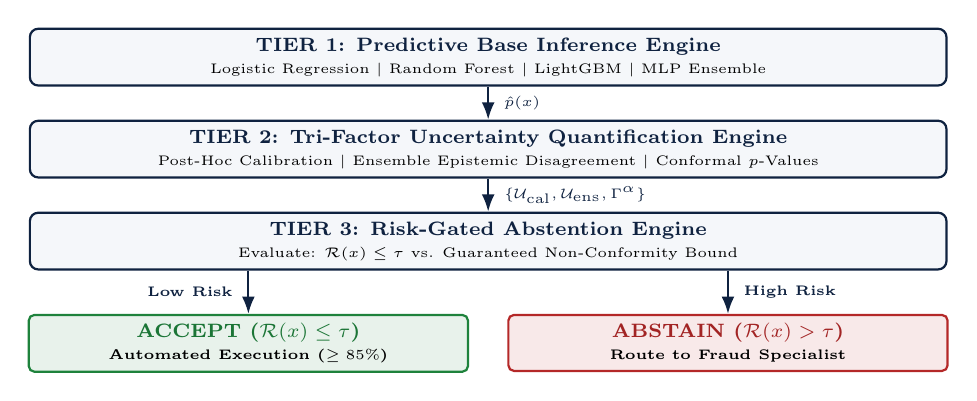
\begin{tikzpicture}[
    box/.style={draw=primary, fill=accentbox, thick, rounded corners=3pt, minimum width=0.96\columnwidth, minimum height=0.72cm, align=center, font=\scriptsize\bfseries, inner sep=3pt},
    outcome/.style={draw, thick, rounded corners=2pt, font=\scriptsize\bfseries, minimum height=0.62cm, minimum width=0.46\columnwidth, align=center, inner sep=3pt},
    arr/.style={-{Latex[length=2.2mm]}, thick, color=primary}
  ]
    % Nodes
    \node [box] (tier1) {\color{primary} TIER 1: Predictive Base Inference Engine \\ \normalfont\tiny Logistic Regression $\vert$ Random Forest $\vert$ LightGBM $\vert$ MLP Ensemble};
    \node [box, below=0.42cm of tier1] (tier2) {\color{primary} TIER 2: Tri-Factor Uncertainty Quantification Engine \\ \normalfont\tiny Post-Hoc Calibration $\vert$ Ensemble Epistemic Disagreement $\vert$ Conformal $p$-Values};
    \node [box, below=0.42cm of tier2] (tier3) {\color{primary} TIER 3: Risk-Gated Abstention Engine \\ \normalfont\tiny Evaluate: $\mathcal{R}(x) \le \tau$ vs. Guaranteed Non-Conformity Bound};
    
    \node [outcome, draw=acceptgreen, fill=acceptgreen!10, below left=0.55cm and 0.02\columnwidth of tier3.south, anchor=north east] (accept) {\color{acceptgreen!90!black} ACCEPT ($\mathcal{R}(x) \le \tau$) \\ \tiny Automated Execution ($\ge 85\%$)};
    \node [outcome, draw=riskalert, fill=riskalert!10, below right=0.55cm and 0.02\columnwidth of tier3.south, anchor=north west] (defer) {\color{riskalert!90!black} ABSTAIN ($\mathcal{R}(x) > \tau$) \\ \tiny Route to Fraud Specialist};

    % Arrows
    \draw [arr] (tier1) -- (tier2) node[midway, right=2pt, font=\tiny\color{gray}] {$\hat{p}(x)$};
    \draw [arr] (tier2) -- (tier3) node[midway, right=2pt, font=\tiny\color{gray}] {$\{\mathcal{U}_{\text{cal}}, \mathcal{U}_{\text{ens}}, \Gamma^\alpha\}$};
    \draw [arr] (tier3.south -| accept.north) -- (accept.north) node[midway, left=2pt, font=\tiny\bfseries\color{acceptgreen!80!black}] {Low Risk};
    \draw [arr] (tier3.south -| defer.north) -- (defer.north) node[midway, right=2pt, font=\tiny\bfseries\color{riskalert!80!black}] {High Risk};
  \end{tikzpicture}%
  }
  \caption{Risk-Aware Selective Classification Pipeline (RASCP) Architecture.}
  \label{fig:rascp_pipeline}
\end{figure}

\subsection{Base Predictive Classifiers (Tier 1)}
To assess model vulnerability across inductive biases, Tier 1 implements:
\begin{itemize}
  \item \textbf{Regularized Logistic Regression (ElasticNet):} Serves as a transparent linear baseline.
  \item \textbf{Random Forest:} Bagged ensemble of decorrelated decision trees producing variance across individual estimators.
  \item \textbf{LightGBM / XGBoost:} Gradient boosted tree ensembles representing state-of-the-art accuracy for tabular classification.
  \item \textbf{Tabular Multi-Layer Perceptron (MLP) \& Deep Ensembles:} Neural baseline trained with Monte Carlo Dropout \cite{gal2016dropout}.
\end{itemize}

\subsection{Tri-Factor Uncertainty Quantification (Tier 2)}
Tier 2 simultaneously estimates aleatoric uncertainty and epistemic ignorance through three complementary mechanisms:
\begin{enumerate}
  \item \textbf{Probability Calibration:} Raw predicted scores $\hat{z}(x)$ are calibrated on held-out validation data via Platt Scaling (logistic sigmoid) and Isotonic Regression \cite{guo2017calibration}:
  \begin{equation}
    \hat{p}_{\text{cal}}(x) = \sigma(a \cdot \hat{z}(x) + b)
  \end{equation}
  \item \textbf{Ensemble Epistemic Disagreement:} Measured across $M$ constituent estimators in the ensemble:
  \begin{equation}
    \mathcal{U}_{\text{ens}}(x) = \frac{1}{M}\sum_{m=1}^M \left(\hat{p}_m(x) - \bar{p}(x)\right)^2
  \end{equation}
  High variance signifies that sub-models disagree due to sparse training support in shifted feature space.
  \item \textbf{Inductive Conformal Prediction:} Given a desired error rate $\alpha \in (0,1)$, we compute non-conformity scores $s_i = 1 - \hat{p}(x_i, y_i)$ on the calibration set. Conformal prediction sets are defined as:
  \begin{equation}
    \Gamma^\alpha(x) = \left\{ y \in \{0, 1\} \;\middle\vert\; 1 - \hat{p}(x, y) \le \hat{q}_{1-\alpha} \right\}
  \end{equation}
  where $\hat{q}_{1-\alpha}$ is the empirical $(1-\alpha)$-quantile of calibration scores \cite{angelopoulos2021gentle}. If $\Gamma^\alpha(x) = \{0, 1\}$, the model is fundamentally ambiguous, triggering abstention.
\end{enumerate}

\subsection{Risk-Gated Abstention Engine (Tier 3)}
Let $g(x) \in \{0, 1\}$ denote the selection function, where $g(x) = 1$ accepts the prediction and $g(x) = 0$ abstains. We formulate a composite risk score:
\begin{equation}
  \begin{split}
    \mathcal{R}(x) = {} & w_1 \left(1 - \max_{y} \hat{p}_{\text{cal}}(y \mid x)\right) \\
    & + w_2 \mathcal{U}_{\text{ens}}(x) + w_3 \mathbb{I}\left(|\Gamma^\alpha(x)| > 1\right)
  \end{split}
\end{equation}
A sample is automated if and only if $\mathcal{R}(x) \le \tau$, where threshold $\tau$ is tuned to guarantee a target automation throughput coverage $c = \mathbb{E}[g(X)] \ge 0.85$.

\subsection{Key Concrete Contributions}
\begin{calloutbox}[title={Project Contributions}]
\begin{enumerate}[leftmargin=1.2em]
  \item \textbf{Controlled Tabular Shift Benchmark:} A turnkey synthesis suite generating four distinct shift modes on financial tabular data.
  \item \textbf{Empirical Uncertainty Bake-Off:} Systematic head-to-head comparison between Platt scaling, ensemble variance, and conformal prediction in tabular domains.
  \item \textbf{Pareto Risk-Coverage Optimization:} Derivation of a cost-optimal abstention frontier balancing false negative liability with human analyst bandwidth.
  \item \textbf{Disentangling OOD from Predictive Risk:} First-principles analysis demonstrating when feature-space anomalies can still be safely automated.
\end{enumerate}
\end{calloutbox}

% =========================================================================
\section{Evaluation Protocol and Performance Metrics}
% =========================================================================

\subsection{Predictive and Calibration Metrics}
Under extreme class imbalance ($0.172\%$), accuracy is uninformative. Models are benchmarked via:
\begin{itemize}
  \item \textbf{AUPRC (Area Under Precision-Recall Curve):} Focuses strictly on the minority fraudulent class.
  \item \textbf{AUROC (Area Under ROC Curve):} Diagnostic power across discrimination thresholds.
  \item \textbf{Expected Calibration Error (ECE):} Partitioning predictions into $K=15$ confidence bins:
  \begin{equation}
    \text{ECE} = \sum_{k=1}^K \frac{|B_k|}{N} \left| \text{acc}(B_k) - \text{conf}(B_k) \right|
  \end{equation}
  \item \textbf{Brier Score:} Mean squared error between probabilities and one-hot labels.
\end{itemize}

\subsection{Selective Classification and Economic Utility}
We evaluate selective classification via:
\begin{itemize}
  \item \textbf{Risk-Coverage Profile \& AURC:} Measuring empirical risk $\mathcal{L}(f, g) = \frac{\sum_{i=1}^N \ell(f(x_i), y_i) g(x_i)}{\sum_{i=1}^N g(x_i)}$ across coverage rates $c \in [0.5, 1.0]$ \cite{geifman2017selective}.
  \item \textbf{Cost-Weighted Financial Utility Function:} Quantifying realistic banking losses:
  \begin{equation}
    \begin{split}
      \text{Total Cost} = {} & C_{\text{FN}} \cdot \text{FN}_{\text{acc}} + C_{\text{FP}} \cdot \text{FP}_{\text{acc}} \\
      & + C_{\text{def}} \cdot N_{\text{def}}
    \end{split}
  \end{equation}
  where parameterized costs reflect standard banking guidelines: $C_{\text{FN}} = \$100$ (fraud loss), $C_{\text{FP}} = \$5$ (customer friction), and $C_{\text{def}} = \$2$ (human analyst triage).
\end{itemize}

\subsection{Comparative Baselines}
\begin{enumerate}
  \item \textbf{Vanilla Classifier:} Standard static threshold $\hat{p} > 0.5$ without abstention.
  \item \textbf{Unsupervised Feature-Space OOD Detector:} Isolation Forest and Mahalanobis Distance flagging outliers in $\mathcal{P}(X)$.
  \item \textbf{Random Abstention Baseline:} Abstaining on random transactions at identical coverage fractions $c$.
\end{enumerate}

\subsection{Quantitative Success Criteria}
\begin{table}[htbp]
  \centering
  \small
  \caption{Quantitative Success Metrics}
  \label{tab:success_criteria}
  \begin{tabularx}{\columnwidth}{lX}
    \toprule
    \textbf{Target Metric} & \textbf{Formal Success Criterion} \\
    \midrule
    \textbf{Cost Reduction} & $\ge 30\%$ lower total financial loss vs. vanilla classifier under Shift A--D. \\
    \textbf{Automation Rate} & Retains $\ge 85\%$ coverage ($c \ge 0.85$) without triggering catastrophic error. \\
    \textbf{Calibration} & ECE $< 0.05$ across all shift test splits post-calibration. \\
    \textbf{Disentanglement} & Proof of non-trivial regions where $\text{OOD}(x)=1$ but $\mathcal{R}(x) \le \tau$. \\
    \bottomrule
  \end{tabularx}
\end{table}

% =========================================================================
\section{Project Roadmap and Timeline}
% =========================================================================
\begin{itemize}
  \item \textbf{Weeks 1--2:} Baseline data ingestion, temporal splitting, and initial classifier benchmark (Logistic Regression, LightGBM).
  \item \textbf{Weeks 3--4:} Implementation of controlled shift injection suite (Covariate, Subpopulation, and Label shift modes).
  \item \textbf{Weeks 5--6:} Integration of Tier 2 uncertainty estimators (Platt scaling, ensemble variance, inductive conformal bounds).
  \item \textbf{Weeks 7--8:} Risk-coverage optimization, financial utility evaluation, error analysis, and final report compilation.
\end{itemize}

% =========================================================================
% References
% =========================================================================
\begin{thebibliography}{9}
  \small
  \bibitem{dalpozzolo2015calibrating}
  A.~Dal Pozzolo, O.~Caelen, R.~A. Johnson, and G.~Bontempi,
  \newblock ``Calibrating probability with undersampling for unbalanced classification,''
  \newblock in \emph{IEEE SSCI}, 2015, pp. 159--166.

  \bibitem{guo2017calibration}
  C.~Guo, G.~Pleiss, Y.~Sun, and K.~Q. Weinberger,
  \newblock ``On calibration of modern neural networks,''
  \newblock in \emph{ICML}, 2017, pp. 1321--1330.

  \bibitem{geifman2017selective}
  Y.~Geifman and R.~El-Yaniv,
  \newblock ``Selective classification for deep neural networks,''
  \newblock in \emph{NeurIPS}, vol.~30, 2017.

  \bibitem{angelopoulos2021gentle}
  A.~N. Angelopoulos and S.~Bates,
  \newblock ``A gentle introduction to conformal prediction and distribution-free uncertainty quantification,''
  \newblock \emph{arXiv:2107.07511}, 2021.

  \bibitem{ovadia2019can}
  Y.~Ovadia et~al.,
  \newblock ``Can you trust your model's uncertainty? Evaluating predictive uncertainty under dataset shift,''
  \newblock in \emph{NeurIPS}, vol.~32, 2019.

  \bibitem{gal2016dropout}
  Y.~Gal and Z.~Ghahramani,
  \newblock ``Dropout as a Bayesian approximation: Representing model uncertainty in deep learning,''
  \newblock in \emph{ICML}, 2016, pp. 1050--1059.
\end{thebibliography}

\end{document}
